\subsection{Analysis and expression of needs}
Researchers from the University of Liège are studying trees in a tropical forest in Gabon to understand how seasonal drought affects the functioning of trees. To achieve their goals, they need a system capable of taking photos twice a day in order to analyze these images later on.
Our objective, as designers of this system, is to create a device that meets the specific requirements of the researchers. The system must be capable of operating in a hot and humid environment, as it will be installed on a pole in a tropical forest. It must also be self-sufficient in terms of energy and storage, as the researchers will only be able to access the system every two or three months.
Furthermore, the system must be able to communicate over long distances to provide researchers with information regarding the sensor data collected. Given that there is no conventional mobile network in the Gabonese forest, this must be done via a decentralized, low-energy, and long-range protocol. However, it will not be possible to send the images directly due to these communication constraints.


%image
\begin{figure}[h]
    \centering
    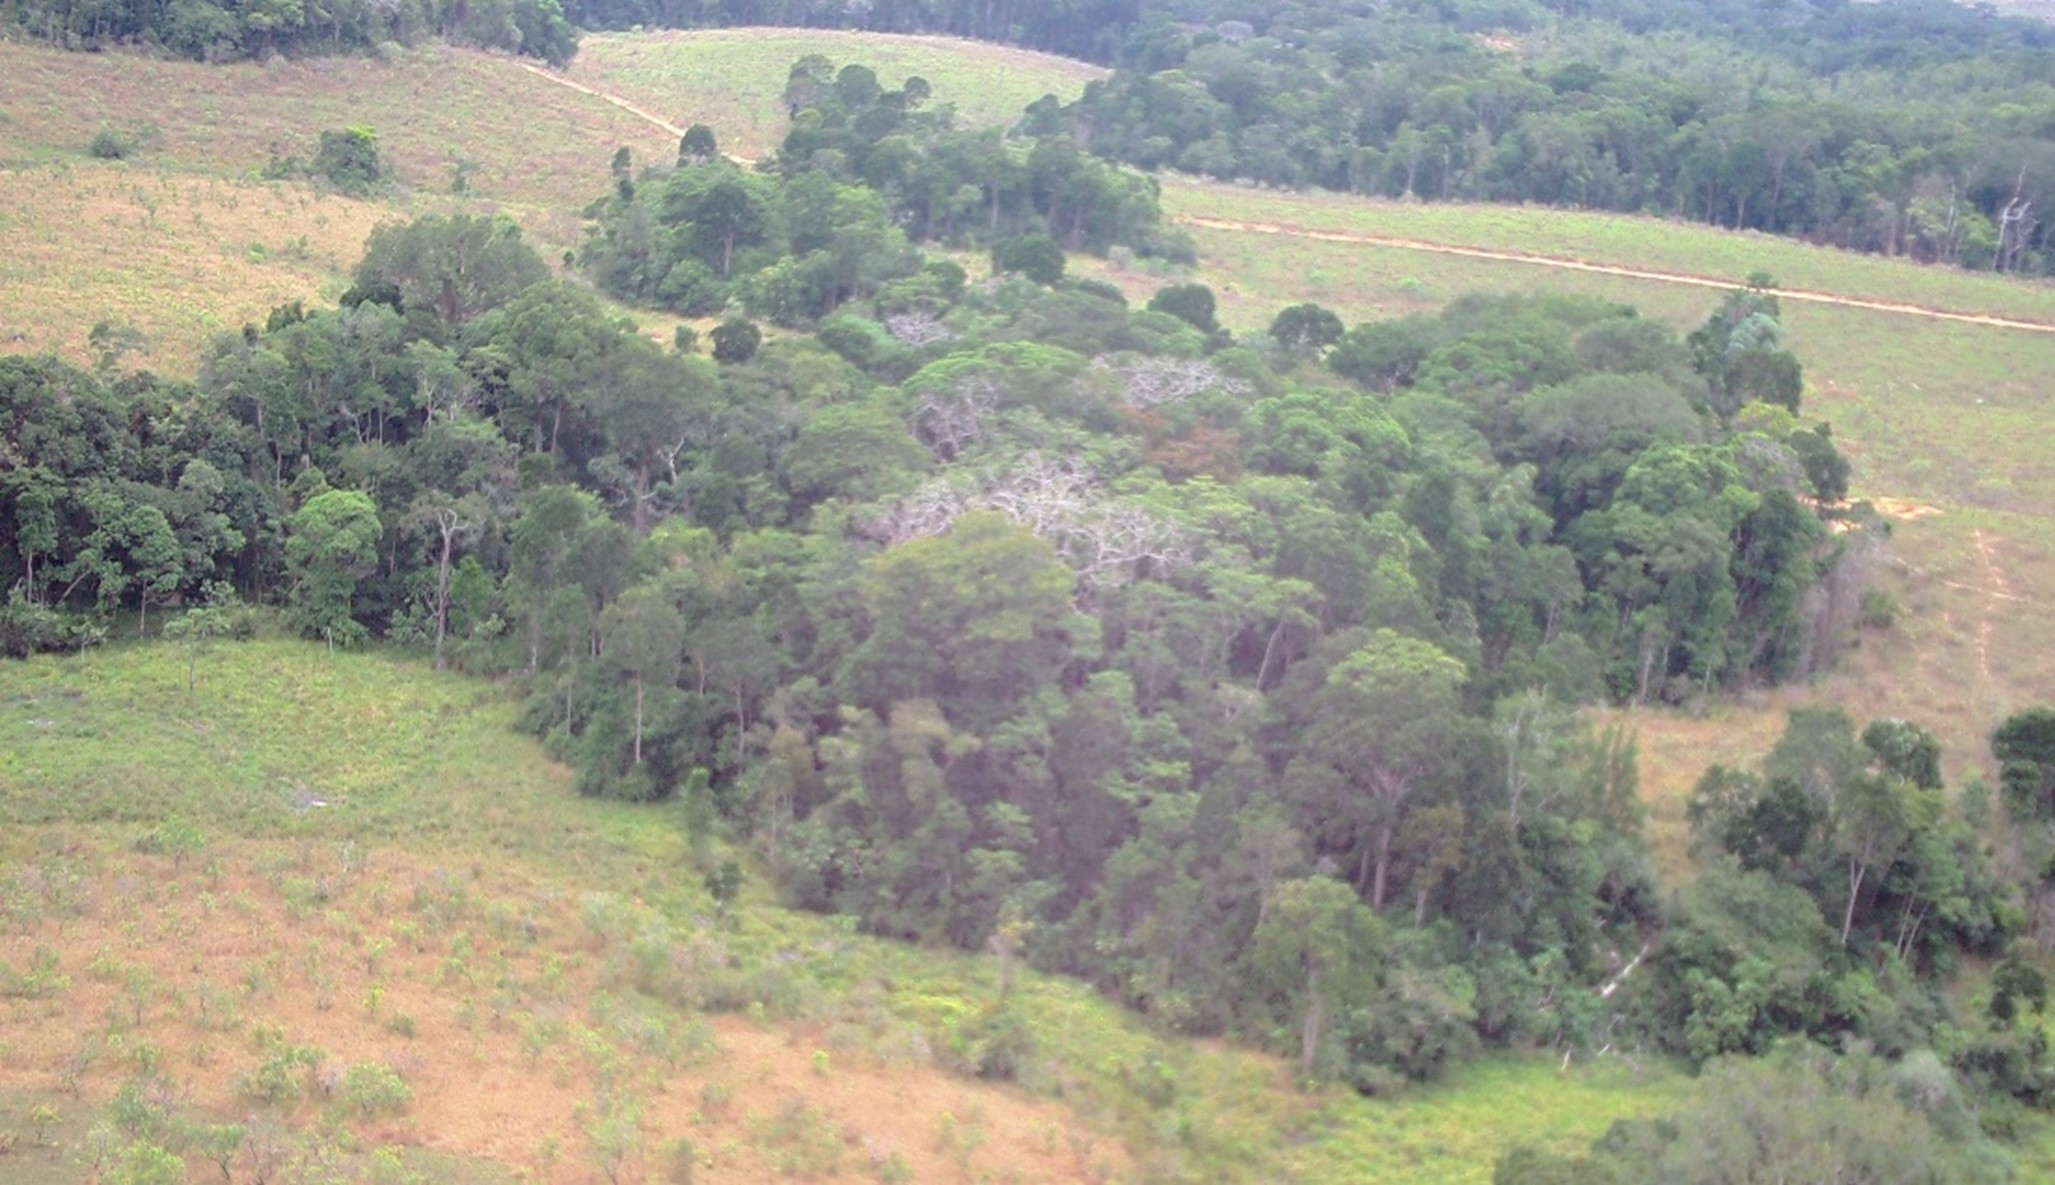
\includegraphics[width=1\textwidth]{\currfiledir/figures/forest.jpg}
    \caption{Example of a picture took by researchers in Gabon}
    \label{fig:forest}
\end{figure}
